\documentclass[11pt,a4paper,dvipdfmx]{article}
%\documentclass[autodetect-engine,dvipdfmx-if-dvi,ja=standard]{bxjsarticle}

\usepackage[utf8]{inputenc}
\usepackage{lmodern}
\usepackage[T1]{fontenc}
\usepackage[noBBpl]{mathpazo}
%\linespread{1.05}
\usepackage{mathtools, amsmath, amssymb, amsthm}
\usepackage{amsfonts}
\usepackage{braket}
%\usepackage{amssymb}
\usepackage{url}
\usepackage{cases}

%% citation
\usepackage[longnamesfirst]{natbib}

%
\theoremstyle{plain}
\newtheorem{thm}{Thm.}[section]
\newtheorem{lem}{Lem.}[section]
\newtheorem{cor}{Cor.}[section]
\newtheorem{prop}{Prop.}[section]
\newtheorem{df}{Def.}[section]
\newtheorem{eg}{e.g.}[section]
\newtheorem{rem}{Rem.}[section]
%

\usepackage{listings}
\lstset{%
language={python},%
basicstyle={\ttfamily\footnotesize},%ソースコードの文字を小さくする
frame={single},
commentstyle={\footnotesize\itshape},%コメントアウトの文字を小さくする
breaklines=true,%行が長くなったときの改行。trueの場合は改行する。
numbers=left,%行番号を左に書く。消す場合はnone。
xrightmargin=3zw,%左の空白の大きさ
xleftmargin=3zw,%右の空白の大きさ
stepnumber=1,%行番号を1から始める場合こうする(たぶん)
numbersep=1zw,%行番号と本文の間隔。
}

%\usepackage[dvipdfmx]{graphicx}
%% color packageとdvipdfmxは相性が悪いらしい
%% https://qiita.com/zr_tex8r/items/442b75b452b11bee8049
\usepackage{graphicx}


\usepackage[left=2cm,right=2cm,top=2cm,bottom=2cm]{geometry} %This changes the margins.
\usepackage{float}
%\author{Kyohei Okumura}
\global\long\def\T#1{#1^{\top}}

\newcommand{\id}{\textnormal{id}}
\newcommand{\R}{\mathbb{R}}
\newcommand{\N}{\mathbb{N}}
\newcommand{\Q}{\mathbb{Q}}
\newcommand{\Z}{\mathbb{Z}}
\newcommand{\C}{\mathbb{C}}
\newcommand{\mF}{\mathcal{F}}
\newcommand{\mG}{\mathcal{G}}
\newcommand{\mA}{\mathcal{A}}
\newcommand{\mB}{\mathcal{B}}
\newcommand{\mC}{\mathcal{C}}
\newcommand{\mD}{\mathcal{D}}
\newcommand{\mL}{\mathcal{L}}
\newcommand{\mM}{\mathcal{M}}
\newcommand{\mO}{\mathcal{O}}
\newcommand{\mP}{\mathcal{P}}
\newcommand{\mS}{\mathcal{S}}
\newcommand{\mT}{\mathcal{T}}
\newcommand{\mV}{\mathcal{V}}
\renewcommand{\Re}{\mathrm{Re}}
\renewcommand{\hat}{\widehat}
\renewcommand{\tilde}{\widetilde}
\renewcommand{\bar}{\overline}
\renewcommand{\epsilon}{\varepsilon}
% \renewcommand{\span}{\mathrm{span}}
\newcommand{\defi}{\stackrel{\Delta}{\Longleftrightarrow}}
\newcommand{\equi}{\Longleftrightarrow}
\newcommand{\s}{\succsim}
\newcommand{\p}{\precsim}
\newcommand{\join}{\vee}
\newcommand{\meet}{\wedge}
\newcommand{\1}{\mbox{1}\hspace{-0.25em}\mbox{l}}

\DeclareMathOperator{\Var}{Var}
\DeclareMathOperator{\Cov}{Cov}
\DeclareMathOperator{\sgn}{sgn}
\DeclareMathOperator{\Card}{Card}
\DeclareMathOperator{\supp}{supp}
\DeclareMathOperator{\Log}{Log}
\DeclareMathOperator{\spn}{span}

\newcommand{\indep}{\mathop{\perp\!\!\!\!\perp}}

\usepackage{color}
\newcommand{\kcomment}[1]{{\textcolor{blue}{#1}}}
\newcommand{\ocomment}[1]{{\textcolor{red}{#1}}}


\begin{document}
\title{SML HW4}
\author{29-176004 奥村 恭平{\footnote{E-mail: kyohei.okumura@gmail.com}
\footnote{東京大学大学院 経済学研究科 M2}
}}
\date{\today}
\maketitle

%%%%%%%%%%%%%%%%%%%%%%%%%%%%%%%%%%%%%%%%%%%%%%%%%%%%%%%%%%%

\section*{宿題1}
記法は断りのない限りスライド中のものをそのまま用いる.$\phi_{ij} := \phi(x_i; \mu_j, \sigma_j)$, $S_e := \sum_{j=1}^m \exp[\gamma_j]$.
$$
l(\theta) := \log L(\theta) = \sum_{i=1}^n
\log
\left[
\sum_{j=1}^m w_j(\gamma_1, \dots, \gamma_m) \phi(x_i; \mu_j, \sigma_j)
\right]
$$

\subsection*{(i) $\hat{w}_k = \frac{1}{n} \sum_{i=1}^n \hat{\eta}_{ik}$}
$\because)$
\begin{equation*}
	\frac{\partial l}{\partial \gamma_k}
	= \sum_i \frac{\sum_j \frac{\partial w_j}{\partial \gamma_k} \cdot \phi_{ij}}{\sum_j w_j \phi_{ij}}
\end{equation*}
ここで,
\begin{align*}
	\sum_j \frac{\partial w_j}{\partial \gamma_k} \cdot \phi_{ij}
	&= - \sum_{j \neq k} \frac{\exp[\gamma_j + \gamma_k]}{S_e^2} \phi_{ij} + \frac{\exp[\gamma_k]S_e - \exp[2 \gamma_k]}{S_e^2} \phi_{ik} \\
	&= - \sum_{j \neq k} w_j w_k \phi_{ij} + (w_k - w_k^2) \phi_{ik} \\
	&= w_k \left[ -\sum_{j=1}^m w_j \phi_{ij} + \phi_{ik} \right]
\end{align*}
であることより,
\begin{align*}
	&\frac{\partial l}{\partial \gamma_k} = 0 \\
	\equi &\sum_i \frac{- \sum_j w_j \phi_{ij} + \phi_{ik}}{\sum_j w_j \phi_{ij}} = 0 \\
	\equi &\sum_i \left[ -1 + \frac{\phi_{ik}}{\sum_j w_j \phi_{ij}} \right] = 0 \\
	\equi &n = \sum_i \frac{\phi_{ik}}{\sum_j w_j \phi_{ij}} \\
	\equi &n \cdot w_k = \sum_i \frac{w_k \phi_{ik}}{\sum_j w_j \phi_{ij}}\\
	\equi &w_k = \frac{1}{n} \sum_i \eta_{ik}
\end{align*}
以上より,(i)の式が示された.

\subsection*{(ii) $\hat{\sigma}_k = \sqrt{\frac{1}{d} \cdot \frac{\sum_i \hat{\eta}_{ik} (x_i - \hat{\mu}_j)^\top (x_i - \hat{\mu}_j)}{\sum_i \hat{\eta}_{ik}}}$}
$\because)$
$s_k := \sigma_k^2$とする.
\begin{equation*}
	\frac{\partial l}{\partial s_k} = \sum_i
	\frac{w_k \frac{\partial \phi}{\partial s_k}}{\sum_j w_j \phi_{ij}}
\end{equation*}
ここで,
\begin{align*}
	\frac{\partial \phi}{\partial s_k}
	&= \frac{\partial}{\partial s_k} \left[
	\frac{1}{(2 \pi s_k)^{\frac{d}{2}}} \exp \left[ - \frac{(x_i - \mu_k)^\top (x_i - \mu_k)}{2 s_k} \right]
	\right] \\
	&= \left[ 2 \pi \left( -\frac{d}{2}\right)
	\frac{1}{(2 \pi s_k)^{\frac{d}{2} + 1}} \exp \left[ - \frac{(x_i - \mu_k)^\top (x_i - \mu_k)}{2 s_k} \right]
	\right] \\
	& \quad + 
	\left[
	\frac{1}{(2 \pi s_k)^{\frac{d}{2}}} \exp \left[ - \frac{(x_i - \mu_k)^\top (x_i - \mu_k)}{2 s_k} \right] \frac{2(x_i - \mu_k)^\top (x_i - \mu_k)}{4 s_k^2}
	\right]
	\nonumber \\
	&= - \frac{d}{2s_k}\phi_{ik} + \frac{(x_i - \mu_k)^\top (x_i - \mu_k)}{2 s_k^2} \phi_{ik}
\end{align*}
であることより,
\begin{align*}
	&\frac{\partial l}{\partial s_k} = 0 \\
	\equi &\sum_i \frac{- \frac{d}{2s_k}w_k \phi_{ik} + \frac{(x_i - \mu_k)^\top (x_i - \mu_k)}{2 s_k^2} w_k \phi_{ik}}{\sum_j w_j \phi_{ij}} = 0 \\
	\equi &\sum_i \frac{- d s_k w_k \phi_{ik} + (x_i - \mu_k)^\top (x_i - \mu_k) w_k \phi_{ik}}{\sum_j w_j \phi_{ij}} = 0 \\
	\equi &\sum_i (- d s_k + (x_i - \mu_k)^\top (x_i - \mu_k)) \eta_{ik} = 0 \\
	\equi &d s_k \sum_i \eta_{ik} = \sum_i (x_i - \mu_k)^\top (x_i - \mu_k) \eta_{ik} \\
	\equi &s_k = \frac{1}{d} \cdot \frac{\sum_i \eta_{ik} (x_i - \mu_k)^\top (x_i - \mu_k)}{\sum_i \eta_{ik}} \\
	\therefore \quad & \sigma_k = \sqrt{\frac{1}{d} \cdot \frac{\sum_i \eta_{ik} (x_i - \mu_k)^\top (x_i - \mu_k)}{\sum_i \eta_{ik}}}
\end{align*}
となり,(ii)の結果を得る.

\subsection*{(iii) $\hat{\mu}_k = \frac{\sum_i \hat{\eta}_{ik} x_i}{\sum_i \hat{\eta}_{ik}}$}
$\because)$
\begin{equation*}
	\frac{\partial l}{\partial \mu_k} = \sum_i
	\frac{w_k \frac{\partial \phi}{\partial \mu_k}}{\sum_j w_j \phi_{ij}}
\end{equation*}
ここで,
\begin{equation*}
	\frac{\partial \phi}{\partial \mu_k} = \phi_{ik} \left[
	- \frac{1}{2 \sigma_k^2} 2 (x_i - \mu_k)
	\right]
\end{equation*}
であるので,
\begin{align*}
	&\frac{\partial l}{\partial \mu_k} = 0 \\
	\equi & \sum_i \frac{(x_i - \mu_k) w_k \phi_{ik}}{\sum_j w_j \phi_{ij}} = 0 \\
	\equi & \sum_i (x_i - \mu_k) \eta_{ik} = 0 \\
	\therefore \quad & \mu_k = \frac{\sum_i \eta_{ik} x_i}{\sum_i \eta_{ik}} 
\end{align*}
となり,(iii)の結果を得る.
\qed


%%%
\section*{宿題2}
末尾のコード(言語はpython)を用いてシミュレーションした.(プロットなどに必要な関数は省略.)上手く元の分布を推定できていることがわかる.

\begin{figure}[H]
  \centering
    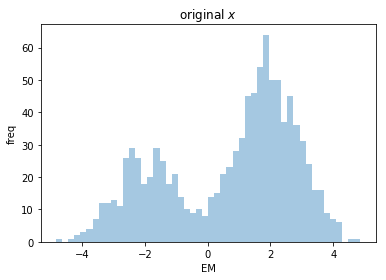
\includegraphics[height=8cm]{image/original_x.png}
    %\caption{\footnotesize $n := 600, \alpha := 0.1$}
    \label{fig:fig1}
\end{figure}
\begin{figure}[H]
  \centering
    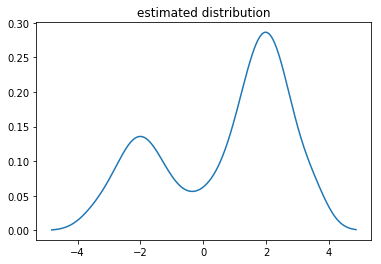
\includegraphics[height=8cm]{image/estimate_x.png}
    %\caption{\footnotesize $n := 600, \alpha := 0.1$}
    \label{fig:fig2}
\end{figure}

\begin{lstlisting}
import numpy as np
import scipy as sp
from numpy.random import randn, rand
from scipy.stats import norm

def em_gauss_sim(n_sample=1000, n_component=5, iter_lim=20, seed=7):
    # set seed
    np.random.seed(seed)

    x = randn(n_sample) + (rand(n_sample) > 0.3) * 4 - 2

    L = - np.inf

    # initial values
    weights = np.ones(n_component) / n_component
    means = np.linspace(np.min(x), np.max(x), n_component)
    covs = np.ones(n_component)/10
    eta = np.zeros([n_sample, n_component])

    # main loop
    n_iter = 0
    while n_iter < iter_lim:
        # E step
        for i in range(n_sample):
            for l in range(n_component):
                eta[i][l] = (weights[l] * norm.pdf(x=x[i], loc=means[l], scale=np.sqrt(covs[l]))) / np.dot(weights, norm.pdf(x=x[i], loc=means, scale=np.sqrt(covs)))

        # M step
        means_prev = means.copy()
        weights_prev = weights.copy()
        covs_prev = covs.copy()
        for l in range(n_component):
            weights[l] = np.sum(eta[:,l]) / n_sample
            covs[l] = np.dot(eta[:,l], (x - means_prev[l])**2) / (1 * np.sum(eta[:,l]))
            means[l] = np.dot(eta[:,l], x) / np.sum(eta[:, l])

        # stop condition
        if np.sum((weights - weights_prev)**2) < 0.00001:
            break

        n_iter += 1

    # for debugging
    print(n_iter)

    sim_x = np.linspace(np.min(x), np.max(x), 1000)
    y = np.zeros_like(sim_x)
    for l in range(n_component):
        tmp = weights[l] * norm.pdf(x=sim_x, loc=means[l], scale=np.sqrt(covs[l]))
        y += tmp

    return x, sim_x, y
\end{lstlisting}

\end{document}